\documentclass[report]{subfiles}
\begin{document}
    \chapter{IMPLEMENTATION}
    The source code for this project can be accessed through the GitHub repository of the project:\\
    \url{https://github.com/Sem-Projects/logic-simulator-inator}
    \section{Brief explanation of the code}
    The source code for our project has been divided into 9 files which consists of 5 C source files and 4 header files. They have been briefly explained below.
    \subsection{component.c \& component.h}
    As the name suggests, these files contain all the necessary information about the components used in the program. The header file defines a structure named Component that encompasses the details about a component including its size, position, input source, number of inputs, input state(s), output state(s) and other information which is later used.
    The output of any component (except clock and state) depends on its input(s). To get the desired output for any component from its inputs, the source file defines different component specific functions. The working of these functions is pretty straight-forward as they follow the standard logic operations available in C. As for the clock, its output is generated based on the value of time variable, which changes as the program progresses, defined in program.c. The clock inverts its current state when time reaches a certain value. The output of state is inverted when the user clicks on it.
    \subsection{draw.h \& draw.c}
    These two files contain the variables and functions that are responsible for drawing all the elements that are visible on the screen such as Buttons, Components, and Wires. It also handles rendering text in the SDL window where necessary. The header file defines an enumeration of confirmation flags that are later used to ask the user for confirmation on certain operations.
    The standard rendering functions available in the SDL library are used in order to draw Buttons and Components. However, SDL does not offer the functionality to draw curves. So, a simple algorithm that approximates a cubic Bezier Curve is used to draw wires.
    As for displaying text, a character map consisting of all the ASCII characters is predefined when the program starts. The font used is robotoo.ttf. The character map is later used to display any text (ASCII based) on the screen.
    \subsection{interaction.h \& interaction.c}
    User interaction is an integral part of any program, even more so for programs that use both mouse and keyboard to take input. These two files are responsible for handling such interactions. The header file defines various structures that are necessary for the Undo/Redo functionalities.
    The source file defines different functions that determine what will happen when a certain button is pressed or when a component is placed on the grid. Since these functions handle interaction with the user, they are usually only called when an event occurs. An SDL event encompasses mouse clicks, keyboard presses, etc. Different functions are called for different events. This coordination is handled in the file program.c.
    \subsection{program.h \& program.c}
    To keep the main.c file clean, the main program loop is defined in this file. For this reason, it acts as the centerpiece of the program that coordinates the functions of all other files. To begin with, the header file defines macros for configuring the main window and different elements inside it. Also, the colors that are frequently used in the program are defined here.
    The source file can be vaguely divided into two parts: Initialization and Main Program Loop. The initialization part is responsible for setting up all the necessary elements needed for the program to function properly. This is a one-time process that occurs when the program is launched.
    The Main Program Loop, as the name suggests, is a loop that runs over and over until the user exits the program. Everything that the user does inside the program is handled in this section. During each loop, the program checks for events, performs necessary operations based on them, updates the elements on the screen if required, and redraws all of those elements.
    \subsection{main.c}
    As mentioned earlier, this file is kept as clean as possible by defining the main loop in program.c. Inside this file, the current working directory is changed to the folder containing the executable and font files, so that the font files are always found regardless of where the program is run from. This is done using the <direct.h> library.
    The main function calls functions for initialization, the main program loop, and finally closing the program.
    
    \section{Rendering}
    There are generally two ways to display graphic elements in an SDL window - displaying images using SDL surfaces or hardware rendering with textures and renderer. This program uses the later as the elements are too versatile to store them as bitmaps.
    \subsection{Render Color}
    Each element on the screen may have a different color. So the renderer stores the color information when drawing anything on the screen. This information is stored if 4 channels commonly known as rgba format. The first three channels indicate intensity of red, green, and blue color respectively. The last channel is used to store the opaqueness of the element. The higher the value the higher the intensity. Before drawing an element on the screen, we must make sure that the renderer is set to the correct color value. This can be done using as shown below.
\begin{lstlisting}
//SDL_SetRenderDrawColor (renderer, red, green, blue, alpha);
SDL_SetRenderDrawColor (renderer, 255, 255, 255, 255);          //opaque white color
\end{lstlisting}
		
    	
    \subsection{Drawing Lines}
    SDL provides direct functionality to draw a straight line between two points. The data doesn't need to be stored anywhere instead we can simply pass the co-ordinates of the points as parameters to the SDL\_RenderDrawLine function and it will draw a line between those points for us. The co-ordinates are relative to the top left point of the window. This function has been used to draw the grid lines and border around the rectangular elements to indicate hovering.
\begin{lstlisting}	
//SDL_RenderDrawLine (renderer, startX, startY, endX, endY);
SDL_SetRenderDrawColor (renderer, 0, 0, 50, 50);            //diagonal line form top left corner
\end{lstlisting}
		
    	
    \subsection{Drawing Rectangles}
    In exchange for the low level access SDL provides, a lot of abstraction has been taken away. A rectangle is arguably the most complicated shape that can be drawn directly from the renderer in SDL. It can either be a rectangular outline or a solid rectangle filled with the current color configurations. In order to do so, the data for a rectangle must be stored using SDL\_Rect structure.
	\begin{figure}[H]
    \centering
    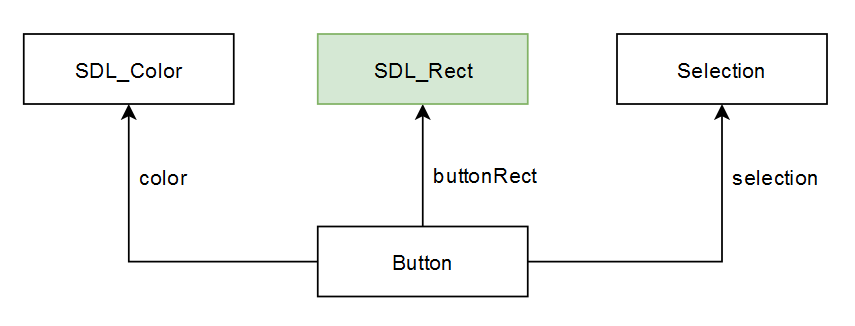
\includegraphics[width=0.8\textwidth]{graphics/button_structure.png}
    \caption{Button Structure}
	\end{figure}
The structure for Button contains a buttonRect element which stores the position and size information for that button. Later, it is used to draw the rectangle as follows:
\begin{lstlisting}
//SDL_RenderFillRect (renderer, &rectangle);
SDL_SetRenderDrawColor (renderer, &Run.buttonRect);            //the rectangle for the Run button
\end{lstlisting}
		
    	
    \subsection{Rendering Text}
    As mentioned earlier, the text rendering is handled by an extension of the SDL library - SDL\_ttf. It provides the functionality to load ttf or rtf fonts and create textures from them. An array of texture pointers is used to store the necessary ASCII characters. A texture is a structure that stores pixel data that can only be accessed through the GPU. Later, this array is used to display any message we want.
\begin{lstlisting}
//display the text stored in message
SDL_Rect dst = {.x = 0, .y = 0, .h = 24};   // h represents the font size
for(int i = 0 ; i < strlen(message); i++){
	//width of each character is different
	dst.w = characterWidth[(int)message[i]]; 
	//display the texture 
	SDL_RenderCopy(renderer, characters[(int)message[i]], NULL, &dst); 
	dst.x += dst.w;           //shift the starting position 
}
\end{lstlisting}
This program uses similar method to display text but with additional functionality to prevent text overflow since the text must stay within the button or component rectangle.

	\subsection{Drawing Wires}
	 Drawing straight lines as wires would clog up the canvas and the circuits would look untidy, so a cubic Bezier curve is used to draw wires. A Bezier curve uses a set of fixed anchor points to draw a curve of certain order. The algorithm to trace such a curve comprises of nested linear interpolation. The level of nesting is determined by the degree of the curve. Here, is an example of a Bezier curve.
	 \begin{figure}[H]
    \centering
    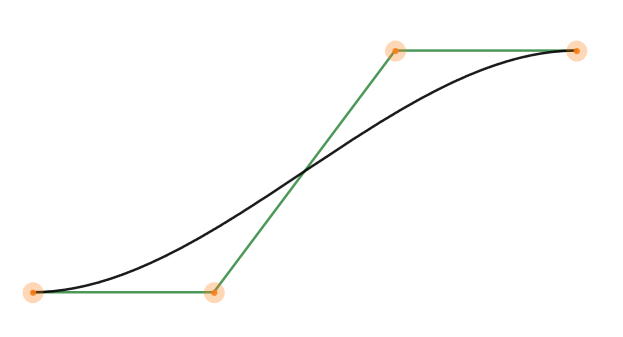
\includegraphics[width=0.8\textwidth]{graphics/bezier_curve.png}
    \caption{Bezier Curve}
	\end{figure}
This can be implemented as follows:
\begin{lstlisting}
// p[4] are the four anchor points
static SDL_Point BezierPoint(float t, SDL_Point p[4])
{
    float tt = t * t;
    float ttt = tt * t;
    float u = 1 - t;
    float uu = u * u;
    float uuu = uu * u;

	//returns a point on the curve for a certain value of t
    return (SDL_Point){
       uuu * p[0].x + 3 * uu * t * p[1].x + 3 * u * tt * p[2].x + ttt * p[3].x,
       uuu * p[0].y + 3 * uu * t * p[1].y + 3 * u * tt * p[2].y + ttt * p[3].y};
}
/* Changing the value of t from 0 to 1 in 100 steps will give 100 points on the curve. We can draw lines between consecutive points to get the desired curve.*/
\end{lstlisting}
    
\end{document}
